\documentclass[english, dvipdfmx, a4paper]{jsarticle}
\usepackage{docmute}
\usepackage[utf8]{inputenc}
\usepackage[top=10truemm, bottom=20truemm, left=15truemm, right=15truemm]{geometry} % mergin
\renewcommand{\headfont}{\bfseries}

% graphics
\usepackage{graphicx}
\usepackage{here}

% link

\usepackage{url}
\usepackage[dvipdfmx, linktocpage]{hyperref} 
\usepackage{xcolor}
\usepackage{pxjahyper}
\hypersetup{
	colorlinks=true,
	citecolor=blue,
	linkcolor=teal,
	urlcolor=orange,
}

% math

\usepackage{amsmath, amssymb} 
\usepackage{physics}
\usepackage{mathrsfs}
\usepackage{mathtools}

% theoremstyle
\usepackage{amsthm}
\newtheoremstyle{break}
{\topsep}{\topsep}%
{}{}%
{\bfseries}{}%
{\newline}{}%
\theoremstyle{break}
\newtheorem{thm}{Theorem}
\newtheorem{defn}[thm]{Definition}
\newtheorem{eg}[thm]{Example}
\newtheorem{cl}[thm]{Claim}
\newtheorem{cor}[thm]{Corollary}
\newtheorem{fact}[thm]{Fact}
\newtheorem{rem}[thm]{Remark}
\newtheorem{prob}{Problem}
\newtheorem{prop}{Property}

\makeatletter
\newenvironment{pr}[1][\proofnam]{\par
\topsep6\p@\@plus6\p@ \trivlist
\item[\hskip\labelsep{\itshape #1}\@addpunct{\bfseries}]\ignorespaces
}{%
\endtrivlist
}
\newcommand{\proofnam}{\underline{Derivation.}}
\makeatother
% ordinary
	\newcommand{\R}{\mathbb{R}}
	\newcommand{\C}{\mathbb{C}}
	\newcommand{\Z}{\mathbb{Z}}
	
	
	% Physics %%%%%%%%%%%%%%%%%%%%%%%%%%%%%%%%%%%%
	
	% Feynman slash
	\newcommand{\slashed}[1]{#1\!\!\!/}
	% order
	
	%Lie algebra
	\renewcommand{\O}{\mathcal{O}}
	\newcommand{\SO}{\mathrm{SO}}
	\newcommand{\so}{\mathfrak{so}}
	\newcommand{\SU}{\mathrm{SU}}
	\newcommand{\su}{\mathfrak{su}}
	\newcommand{\SP}{\mathrm{SP}}
	\renewcommand{\sp}{\mathfrak{sp}}
	\newcommand{\SL}{\mathrm{SL}}
	\renewcommand{\sl}{\mathfrak{sl}}
	\newcommand{\GL}{\mathrm{GL}}
	\newcommand{\gl}{\mathfrak{gl}}
	\newcommand{\U}{\mathrm{U}}
	\renewcommand{\u}{\mathfrak{u}}
\renewcommand{\i}{\mathrm{i}}
\newcommand{\e}{\mathrm{e}}
\newcommand{\N}{\mathcal{N}}
\newcommand{\Q}{\mathcal{Q}}
\renewcommand{\P}{\mathcal{P}}
\renewcommand{\S}{\text{S}}
% number

%\makeatletter
%\@addtoreset{equation}{section}
%\makeatother
%\numberwithin{equation}{section}
\renewcommand{\thefootnote}{\roman{footnote}.}
\renewcommand{\appendixname}{Appendix }

\title{SUSYQM}
\author{Toshiya Tanaka}
\date{\today}

\begin{document}
	\begin{eg}[調和振動子]
		$W(x)\coloneqq m\omega x^2/2$とすると
		\begin{equation}
			H_{\pm} = -\frac{\hbar^2}{2m}\dv[2]{}{x} + \frac{m\omega^2}{2}x^2 \mp \frac{\hbar\omega}{2}
		\end{equation}
		となり,調和振動子を$\pm\hbar\omega/2$ずつずらしたかたちのHamiltonianになって,これらが超対称パートナーになっている.

		定義どおり,計算すると,
		\begin{equation}
			A = \frac{-\i m\omega}{\sqrt{2m}}\qty(x - \frac{\hbar}{m\omega}\dv{}{x}) = -\i \sqrt{\hbar\omega}\ a
		\end{equation}
		になっている.ここで$a$は通常の消滅演算子になっていて,$a = \sqrt{m\omega/(2\hbar)}(x + \hbar/(m\omega)\dv*{}{x})$である.

		Hamiltonianは
		\begin{equation}
			H = 
			\mqty(\hbar\omega a^{\dag}a & 0 \\
			0 & \hbar\omega aa^{\dag})
		\end{equation}
		である.エネルギー固有値は$E_{n, +} = n\hbar\omega,\ (n\in\Z_{\geq0})$, $E_{n, -} = n\hbar\omega,\ (n\in\Z_{>0})$であり,ゼロエネルギー状態は$H_+$の方に存在する.
		ゼロエネルギー状態は$a\psi_{0, +}(x) = 0$の解であり,$\psi_{0, +}(x) = N_{0, +}\e^{-m\omega x^2/(2\hbar)}$である.


		$H_{-}a\psi_{n, +}(x) = \hbar\omega(aa^{dag}a)\psi_{n, +}(x) = aH_+\psi_{n, +}(x) = n\hbar\omega a\psi_{n, +}(x)$であることから,$a$は$H_+$の固有状態を$H_-$の固有状態に移すことがわかる.$a^{\dag}$についても同様.
	\end{eg}
	
	\begin{eg}[自由粒子とRosen--Morseポテンシャル]
		$W'(x) = \hbar\tanh(x)$と選ぶと
		\begin{align}
			V_+(x) &= \frac{\hbar^2}{2m}\qty(1-\frac{2}{\cosh^2(x)})\\
			V_-(x) &= -\frac{\hbar^2}{2m}
		\end{align}
		となる.$V_+$の方をRosen--Morseポテンシャルといい,$V_-$は定数ずれた自由粒子である.
	\end{eg}

	\begin{eg}[$\delta$関数ポテンシャル]
		$W'(x) = \alpha\hbar(\Theta(x) - \Theta(-x))$で与えると,
		$V_{\pm}(x) = \hbar^2/(2m)(\alpha^2 \mp 2\alpha\delta(x))$となる.
	\end{eg}

	\begin{eg}[Coulombもどき]
		$W'(x) = me^2/(\hbar l) - \hbar l/x$, $(x>0)$で与えると,
		\begin{equation}
			V_{\pm}(x) = -\frac{e^2}{x} + \frac{\hbar^2l(l\mp1)}{x^2} + \frac{me^2}{2\hbar^2l^2}
		\end{equation}
		となる\footnote{若干違うが,水素の動径方向に似ている.}.軌道角運動量が$l$のものと$l-1$のものがパートナーになっていると思える.
	\end{eg}

	\begin{eg}[Dirichlet and Neumann boundary condition]
		$-1 \leq x \leq 1$に制限した有限系を考える.$V_{\pm}(x) = 0$として,境界条件を$\psi'_{E, +}(-1) = \psi'_{E, +}(1) = 0$と$\psi_{E, -}(-1) = \psi_{E, -}(1) = 0$と入れた二つの系を考える.前者をNeunamm, 後者をDirichlet境界条件という.
		$A = -\i\hbar/\sqrt{2m}\dv*{}{x}$なので,これらは両者を移し合う.

		このように,境界条件を変えた系を移し合うケースもある\footnote{境界条件のSUSYによる対応は\href{https://arxiv.org/abs/0812.4659}{arXiv:0812.4659}に詳しい.}.
	\end{eg}

	\begin{eg}[無限に深い井戸型ポテンシャル]
		$W'(x) = \hbar\tan(x), \ (-\pi/2\leq x\leq \pi/2)$とすると,$V_+(x) = -\hbar^{2}/(2m)$, $V_-(x) = \hbar^2/(2m)(2/\cos^2(x) - 1)$となる.後者をP\"{o}schl--Tellerポテンシャルという.
	\end{eg}
	
	超対称パートナーは同じエネルギースペクトラムがあるが,ポテンシャルの形を見ただけでその対応を読み取るのは困難である.例として,自由粒子とRosen--Morse,井戸型とP\"{o}schl--Tellerを図示してみた (Fig. \ref{fig:Rosen-Morse}, \ref{fig:Poeschl-Teller}).
	非自明な対応がSUSYを通して理解できることがわかる.
		\begin{figure}[t]
			\centering
			\begin{tabular}{cc}
				\begin{minipage}[t]{0.45\hsize}
					\centering
					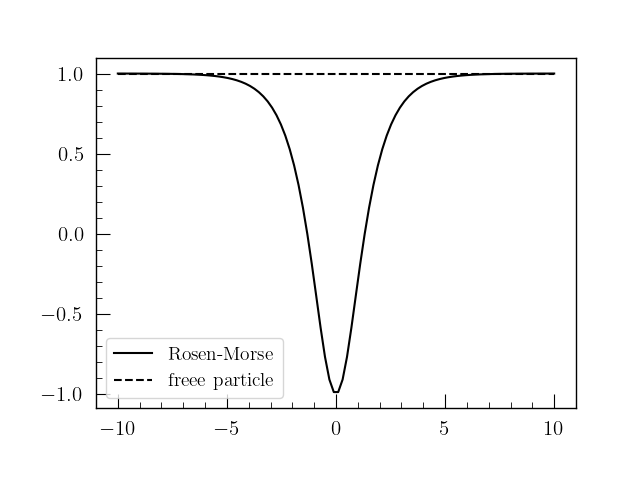
\includegraphics[width=6cm]{./potentials/free-RM.png}
					\caption{自由粒子とRosen--Morseポテンシャルの比較.}
					\label{fig:Rosen-Morse}
				\end{minipage}&
				\begin{minipage}[t]{0.45\hsize}
					\centering
					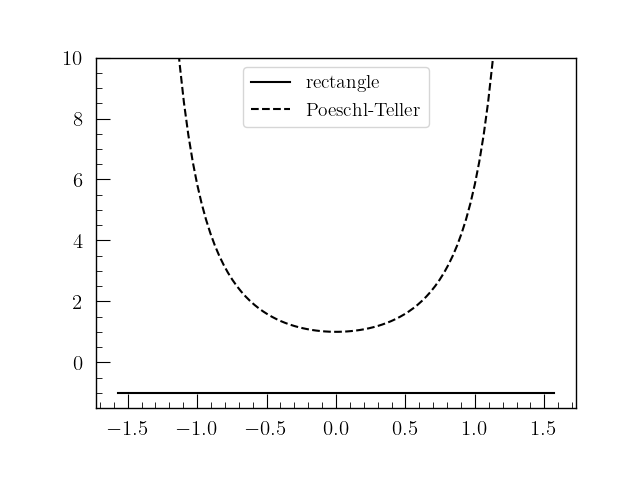
\includegraphics[width=6cm]{./potentials/rectangle-PT.png}
					\caption{井戸型ポテンシャルとP\"{o}schl--Tellerポテンシャルの比較.}
					\label{fig:Poeschl-Teller}
				\end{minipage}
			\end{tabular}
		\end{figure}

	\section{Exactly solvable model}
	\subsection{超対称関係からの視点}
	\begin{defn}[Exactly solvable]
		Exactly solvableとは,量子力学系のエネルギー固有値と固有関数がすべてわかることを指す.
	\end{defn}
	
	\begin{thm}\label{thm:construct_by_groundstate}
		一次元量子力学系でground state $\psi_0(x)$とground energy $E_0$が与えられているとする.
		このとき,
		\begin{align}
			W'(x) &\coloneqq -\hbar \psi_0(x)/\psi_0(x)\label{eq:Wp_solv}\\
			A & \coloneqq -\frac{\i\hbar}{\sqrt{2m}}\qty(\dv{}{x} + \frac{1}{\hbar}W'(x))\label{eq:A_solv}\\
			A^{\dag} &= -\frac{\i\hbar}{\sqrt{2m}}\qty(\dv{}{x} - \frac{1}{\hbar}W'(x))
		\end{align}
		とすると,Hamiltonianは$H = A^{\dag}A + E_0$となる.

		また,$A\psi_0(x) = 0$を満たす.
	\end{thm}

	量子力学なので,Hamiltonianは$H = -\hbar^2/(2m)\dv*[2]{}{x} + V(x)$である.Ground stateに関して,$H\psi_0(x) = E_0\psi_0(x)$なので,
	\begin{equation}
		V(x) = \frac{\hbar^2}{2m}\frac{\psi_0''(x)}{\psi_0(x)} + E_0
	\end{equation}
	である.
	部分積分をすると,$\hbar^2\psi_0''(x)/\psi_0(x) = -\hbar W''(x) +(W'(x))^2$だから
	\begin{equation}
		V(x) = \frac{1}{2m}W'(x) - \frac{\hbar}{2m}W''(x) + E_0\label{eq:SUSY_potential}
	\end{equation}
	となる.よって,Eq. \eqref{eq:A_solv}のように$A$を設定すれば,$H = A^{\dag}A + E_0$となる.

	また,定義から計算すれば,$A\psi_0(x) = 0$となる.\qed

	Theorem. \ref{thm:construct_by_groundstate}では$W'(x)$を一つ与え,
	Eq. \eqref{eq:SUSY_potential}の形の$V(x)$を求めたが,
	この形のポテンシャルをつくる$W'(x)$がわかれば,同様の手法で解を構成できる.
	次は,ポテンシャル
	\begin{equation}
		V_{(1)}(x) = \frac{1}{2m}(W'(x))^2 -\frac{\hbar}{2m}W''(x)
	\end{equation}
	が与えられたとき,これを$W'(x)$について解いて,他の可解量子力学系を構成する方法を考える.
	この非線形な微分方程式はRiccati型として知られており,
	$\phi(x) \coloneqq \e^{-W(x)/\hbar}$とおくことで,Schr\"{o}dinger型の微分方程式
	\begin{equation}
		-\frac{\hbar^2}{2m}\dv[2]{\phi(x)}{x} + V_{(1)}(x)\phi(x) = \mathcal{E}_{(1)}\phi(x)\label{eq:Riccati_Schroedinger}
	\end{equation}
	に線形化できる.ここで,$\mathcal{E}_{(1)}$は$\mathcal{E}_{(1)} < E_0$を満たす\footnote{$A^{\dag}A$の形にする以上,固有値は必ず非負になる.最低エネルギーが$E_0$にシフトしたので,この場合に非負という条件はこのようになる.}ように取れるパラメータである\footnote{パラメータはこの条件を満たしても,superpotentialの素性が悪くなる(発散したりする)こともあるようである.そうならない範囲でパラメータは自由に取れる.}.
	\begin{thm}
		今,Eq. \eqref{eq:Riccati_Schroedinger}の特解を$\phi_{\S}(x)$を用いて,一般解は
		\begin{equation}
			W_{(1)}'(x) = -\hbar \frac{\phi_{\S}'(x)}{\phi_\S(x)} - \frac{\hbar(\phi_\S(x)^{-2})}{c_{(1)} + \displaystyle\int_{x_0}^{x}\dd{z}(\phi_{\S}(z))^{-2}}
		\end{equation}
		とかける.
	\end{thm}
	$\phi(x)\coloneqq \rho(x)\phi_\S(x)$とする.Eq. \eqref{eq:Riccati_Schroedinger}に代入すると,
	$\rho''(x)\phi_\S(x) + 2\rho'(x)\phi'_\S(x) = 0$を満たすことがわかる.今,$\rho'(x)\phi_\S(x)$でわって,
	\begin{equation}
		\frac{\rho''(x)}{\rho'(x)} + \frac{2\phi_\S'(x)}{\phi_\S(x)} = \dv{}{x} \qty(\log \rho'(x)(\phi_\S(x))^2)
	\end{equation}
	なので,
	\begin{equation}
		\rho(x) = c_1 + \int_{x_0}^{x}\dd{z}c_0(\phi_\S(x))^{-2}
	\end{equation}
	となる.$c_0$, $c_1$は積分定数である.

	定義をたどって,元に戻すと,
	\begin{equation}
		W'(x) = - \hbar\frac{\phi'_\S(x)}{\phi_\S(x)} - \frac{\hbar(\phi_\S(x))^{-2}}{c_1/c_0 + \int_{x_0}^{x}\dd{z}(\phi_\S(z))^{-2}}
	\end{equation}
	となり,$c_{(1)} = c_1/c_0$と置くことで示せる.\qed


	以上より求まった,$W'_{(1)}(x)$を用いて,$A_{(1)}$を定めることでHamiltonianは$H_{(1)} = A_{(1)}^\dag A_{(1)} + \mathcal{E}_{(1)}$となり,エネルギースペクトラムが同じの超対称パートナーは
	$H_{(2)} = A_{(1)}A_{(1)}^{\dag} + \mathcal{E}_{(1)}$となる.$H_{(1)}$がexactly solvableなら$H_{(2)}$についても完全にわかったことになる.
	また,$H_{(2)}$も量子力学のHamiltonianなので,$H_{(2)} = A_{(2)}^{\dag}A_{(2)} + \mathcal{E}_{(1)} + \mathcal{E}_{(1)}$とできる.ここから$H_{(3)}$が作れるなど,この操作を繰り返したくさんの可解量子力学系のfamilyを作ることができる.
\end{document}
